\documentclass[border=0pt]{standalone}
\newcommand{\revlamina}{1}
\providecommand{\revlamina}{1}
% Preámbulo común de las láminas VE (A3 horizontal, 420 x 297 mm)
\usepackage[T1]{fontenc}
\usepackage[utf8]{inputenc}
\usepackage[spanish,es-nodecimaldot]{babel}
\usepackage[scaled=0.92]{helvet}
\renewcommand{\familydefault}{\sfdefault}
\usepackage{tikz}
\usetikzlibrary{arrows.meta,patterns,calc,babel,positioning,decorations.pathreplacing}
\usepackage{siunitx}
\sisetup{output-decimal-marker={,},mode=text}
\DeclareSIUnit\kWp{kWp}
\DeclareSIUnit\ohm{\ensuremath{\Omega}}

\definecolor{inv1}{RGB}{37,99,180}
\definecolor{inv2}{RGB}{22,128,84}
\definecolor{nfpa}{RGB}{200,30,30}
\definecolor{viento}{RGB}{40,70,200}
\definecolor{sombra}{RGB}{230,130,0}
\definecolor{losa}{RGB}{120,190,200}
\definecolor{dc}{RGB}{225,95,0}
\definecolor{exist}{RGB}{110,110,110}
\definecolor{nuevo}{RGB}{190,20,20}

% Marcador de referencia numerada
\newcommand{\refm}[2]{\node[circle,draw=black,fill=white,line width=0.35pt,inner sep=0pt,minimum size=3.4mm,font=\fontsize{5.5}{6}\selectfont\bfseries] at #1 {#2};}

% Cajetín: \cajetin{lamina}{titulo}{contenido}{escala}{hoja}
\newcommand{\cajetin}[5]{%
  \draw[line width=0.6pt] (250,10) rectangle (410,58);
  \draw[line width=0.3pt] (250,46) -- (410,46);
  \draw[line width=0.3pt] (250,34) -- (410,34);
  \draw[line width=0.3pt] (250,22) -- (410,22);
  \draw[line width=0.3pt] (370,10) -- (370,34);
  \draw[line width=0.3pt] (330,10) -- (330,22);
  \node[anchor=north west,font=\fontsize{6}{7}\selectfont,align=left] at (251.5,57) {\textbf{Instituto Tecnológico de Costa Rica} -- EL-4601 Normalización Técnica para Electrónica\\Proyecto No.~3: Cargadores para vehículos eléctricos -- diseño en Costa Rica};
  \node[anchor=north west,font=\fontsize{6}{7}\selectfont,align=left] at (251.5,45) {\textbf{Proyecto:} Estación de carga VE de uso público -- Parqueo norte, campus UTN Villa Bonita (CAA-TEC)\\\textbf{Propietario:} Universidad Técnica Nacional -- Catastro A-652521-2000};
  \node[anchor=north west,font=\fontsize{6.5}{7.5}\selectfont,align=left,text width=115mm] at (251.5,33) {\textbf{Contenido:} #2\\#3};
  \node[anchor=north west,font=\fontsize{5.5}{6.5}\selectfont,align=left] at (371.5,33) {\textbf{Lámina}};
  \node[font=\fontsize{16}{18}\selectfont\bfseries] at (390,25.5) {#1};
  \node[anchor=north west,font=\fontsize{5.5}{6.5}\selectfont,align=left] at (251.5,21) {\textbf{Elaboró:} Grupo de trabajo EL-4601\\\textbf{Revisó:} \rule{25mm}{0.2pt}\\\textbf{Fecha:} 3/11/2026 \quad \textbf{Rev.:} \revlamina};
  \node[anchor=north west,font=\fontsize{5.5}{6.5}\selectfont,align=left] at (331.5,21) {\textbf{Escala (A3):}\\#4};
  \node[anchor=north west,font=\fontsize{5.5}{6.5}\selectfont,align=left] at (371.5,21) {\textbf{Hoja:}\\#5};
}
% Marco de la lámina
\newcommand{\marco}{%
  \draw[line width=0.2pt,white] (0,0) rectangle (420,297);
  \draw[line width=0.8pt] (10,10) rectangle (410,287);
}

\definecolor{ac}{RGB}{37,99,180}
\definecolor{gbt}{RGB}{22,128,84}
\definecolor{dcc}{RGB}{225,95,0}
\definecolor{ali}{RGB}{190,20,20}
\definecolor{tierra}{RGB}{30,140,60}

\begin{document}
\begin{tikzpicture}[x=1mm,y=1mm]
\marco
\node[anchor=north west,inner sep=0pt] at (15.00,283.00) {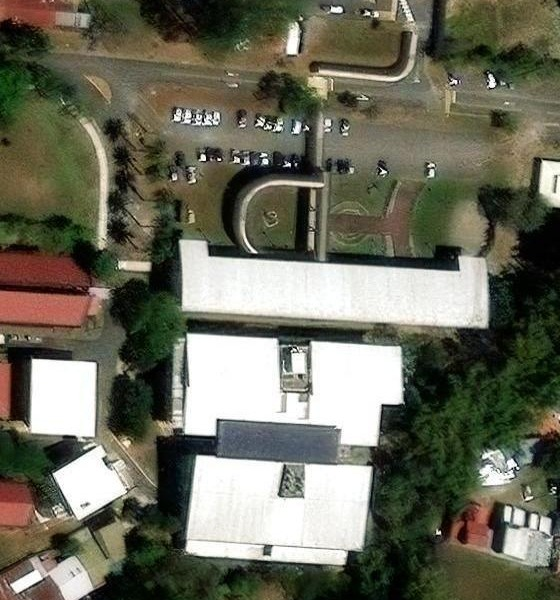
\includegraphics[width=200.0mm]{ve00_base.jpg}};
\draw[line width=0.4pt] (15.00,283.00) rectangle ++(200.0,-214.29);
\draw[ali,line width=1.6pt,dash pattern=on 3pt off 1.5pt] (166.79,129.43) -- (193.57,133.71) -- (193.57,218.00) -- (174.29,218.00) -- (174.29,221.57);
\draw[yellow,line width=1.2pt,fill=yellow,fill opacity=0.25] (148.93,230.14) rectangle (170.36,221.57);
\filldraw[ali,draw=black,line width=0.3pt] (171.76,224.51) rectangle ++(2.2,-1.6);
\draw[yellow!70!black,line width=0.5pt] (159.64,225.86) -- (120.00,276.50);
\filldraw[yellow!70!black,draw=black,line width=0.3pt] (159.64,225.86) circle (1.0);
\node[anchor=west,fill=white,draw=yellow!70!black,line width=0.4pt,inner sep=1.2pt,font=\fontsize{6}{7}\selectfont,text width=60mm] at (120.00,278.00) {\textbf{1}~ Estación de carga VE (VE-01): 4 puntos CA + 1 cargador CC de 60 kW (2 conectores)};
\draw[ali,line width=0.5pt] (172.86,223.71) -- (150.00,266.50);
\filldraw[ali,draw=black,line width=0.3pt] (172.86,223.71) circle (1.0);
\node[anchor=west,fill=white,draw=ali,line width=0.4pt,inner sep=1.2pt,font=\fontsize{6}{7}\selectfont,text width=60mm] at (150.00,268.00) {\textbf{2}~ Celda eléctrica: TD-VE, T-VE 45 kVA, TD-AC, paro de emergencia};
\draw[ali,line width=0.5pt] (166.79,129.43) -- (150.00,118.50);
\filldraw[ali,draw=black,line width=0.3pt] (166.79,129.43) circle (1.0);
\node[anchor=west,fill=white,draw=ali,line width=0.4pt,inner sep=1.2pt,font=\fontsize{6}{7}\selectfont,text width=60mm] at (150.00,120.00) {\textbf{3}~ Transformador ICE N.\textsuperscript{o} 119688, 750 kVA, 34,5 kV/480Y/277 V, y nicho con IP-VE 200 A (posición según E01, aprox.)};
\draw[ali,line width=0.5pt] (193.57,175.86) -- (150.00,148.50);
\filldraw[ali,draw=black,line width=0.3pt] (193.57,175.86) circle (1.0);
\node[anchor=west,fill=white,draw=ali,line width=0.4pt,inner sep=1.2pt,font=\fontsize{6}{7}\selectfont,text width=60mm] at (150.00,150.00) {\textbf{4}~ Alimentador AL-VE: 3\#3/0 + N\#4 + EGC\#6 Cu en PVC 3'' + ducto de reserva, $\approx$111 m medidos (se adoptan 120 m)};
\draw[exist,line width=0.5pt] (46.43,111.57) -- (40.00,98.50);
\filldraw[exist,draw=black,line width=0.3pt] (46.43,111.57) circle (1.0);
\node[anchor=west,fill=white,draw=exist,line width=0.4pt,inner sep=1.2pt,font=\fontsize{6}{7}\selectfont,text width=55mm] at (40.00,100.00) {\textbf{5}~ Edificio CAA-TEC (Proyecto 2)};
\draw[exist,line width=0.5pt] (118.57,140.14) -- (60.00,128.50);
\filldraw[exist,draw=black,line width=0.3pt] (118.57,140.14) circle (1.0);
\node[anchor=west,fill=white,draw=exist,line width=0.4pt,inner sep=1.2pt,font=\fontsize{6}{7}\selectfont,text width=55mm] at (60.00,130.00) {\textbf{6}~ Nave UTN (existente)};
\draw[exist,line width=0.5pt] (104.29,256.21) -- (40.00,276.50);
\filldraw[exist,draw=black,line width=0.3pt] (104.29,256.21) circle (1.0);
\node[anchor=west,fill=white,draw=exist,line width=0.4pt,inner sep=1.2pt,font=\fontsize{6}{7}\selectfont,text width=55mm] at (40.00,278.00) {\textbf{7}~ Calle interna del campus (acceso vehicular a la estación)};
\draw[exist,line width=0.5pt] (107.86,225.86) -- (40.00,266.50);
\filldraw[exist,draw=black,line width=0.3pt] (107.86,225.86) circle (1.0);
\node[anchor=west,fill=white,draw=exist,line width=0.4pt,inner sep=1.2pt,font=\fontsize{6}{7}\selectfont,text width=55mm] at (40.00,268.00) {\textbf{8}~ Parqueo existente de la UTN (asfalto, espacios a 90°)};
\draw[-{Latex[length=3mm]},line width=1.2pt,white] (14.14,256.21) -- ++(10,0);
\node[font=\fontsize{5.5}{6}\selectfont\bfseries,white,anchor=south west] at (14.14,256.81) {acceso};
\begin{scope}[shift={(205.00,80.71)}]
\filldraw[fill=white,draw=black,line width=0.4pt] (0,0) circle (6);
\fill[black] (0,5.2) -- (-2.2,-3.8) -- (0,-2.2) -- cycle; \draw[black,line width=0.4pt,fill=white] (0,5.2) -- (2.2,-3.8) -- (0,-2.2) -- cycle;
\node[font=\fontsize{8}{9}\selectfont\bfseries] at (0,8.2) {N};
\end{scope}
\foreach \i in {0,1,2,3}{\filldraw[fill=\ifodd\i white\else black\fi,draw=black,line width=0.3pt] (15.00+\i*24.295,60.71) rectangle ++(24.295,1.6);}
\node[font=\fontsize{5.5}{6}\selectfont,anchor=north] at (15.00,60.21) {0};
\node[font=\fontsize{5.5}{6}\selectfont,anchor=north] at (39.30,60.21) {20};
\node[font=\fontsize{5.5}{6}\selectfont,anchor=north] at (63.59,60.21) {40};
\node[font=\fontsize{5.5}{6}\selectfont,anchor=north] at (87.89,60.21) {60};
\node[font=\fontsize{5.5}{6}\selectfont,anchor=north] at (112.18,60.21) {80};
\node[font=\fontsize{5.5}{6}\selectfont,anchor=west] at (114.18,61.51) {m (escala gráfica, $\pm$5 \%)};
\node[anchor=north west,font=\fontsize{9}{11}\selectfont\bfseries] at (222,283) {DATOS DEL EMPLAZAMIENTO};
\node[anchor=north west,font=\fontsize{6.2}{7.8}\selectfont,align=left,text width=180mm] at (222,276) {%
\begin{tabular}{@{}p{38mm}p{140mm}@{}}
Provincia / cantón & Alajuela / Alajuela (Central), Sede Central UTN, Villa Bonita ($\approx$960 msnm)\\
Coordenadas de la estación & 10,0065\,°N; 84,2155\,°O (imagen satelital, $\pm$10 m)\\
Propietario / usuario & Universidad Técnica Nacional (catastro A-652521-2000) / comunidad universitaria UTN--TEC y visitantes\\
Uso & Estación de carga de uso público en parqueo institucional (acceso controlado con tarjeta RFID o aplicación)\\
Distribuidora & ICE. Transformador de pedestal N.\textsuperscript{o} 119688, 750 kVA, 34,5 kV/480Y/277 V (lámina E01 del CAA)\\
Servicio nuevo & 480Y/277 V, 3F 4H, medición indirecta del ICE independiente del CAA, IP-VE 200 A\\
Puntos de carga & AC-1, AC-2: CA 208 V, J1772, 8,3 kW (40 A) $\cdot$ AC-3, AC-4: CA 208 V, GB/T, 6,7 kW (32 A)\\
 & DC-1: CC 60 kW, CCS1 + CHAdeMO (30 + 30 kW con dos vehículos)\\
Demanda máxima & 94,5 kW sin gestión; 60 kW con el sistema de gestión de carga (NEC 625.42)\\
\end{tabular}};
\node[anchor=north west,font=\fontsize{9}{11}\selectfont\bfseries] at (222,216) {ÍNDICE DE LÁMINAS};
\node[anchor=north west,font=\fontsize{6.4}{8}\selectfont,align=left] at (222,209) {%
\textbf{VE-00}\quad Plano general de ubicación (esta lámina)\\
\textbf{VE-01}\quad Planta de la estación: puntos de carga, estacionamientos, celda eléctrica, canalizaciones y accesos (1:100)\\
\textbf{VE-02}\quad Diagrama unifilar desde el transformador del ICE hasta cada cargador\\
\textbf{VE-03}\quad Detalles de montaje, zanja, puesta a tierra, rotulación y medidas de emergencia};
\node[anchor=north west,font=\fontsize{9}{11}\selectfont\bfseries] at (222,180) {NOTAS};
\node[anchor=north west,font=\fontsize{6.2}{7.6}\selectfont,align=left,text width=183mm] at (222,173) {%
1. Imagen base: Esri World Imagery (Maxar), nivel de zoom 19, descargada el 1/11/2026; resolución 0,29 m/px. Norte arriba.\\
2. La posición del transformador del ICE y del nicho de 480 V se transcribió de la lámina E01 (as-built del CAA, Proyecto 2); en la imagen queda bajo vegetación y debe confirmarse en sitio (supuesto S).\\
3. La ruta del alimentador evita la nave y los árboles: va por el costado este de la nave y por el borde del parqueo. Longitud medida $\approx$111 m; se adoptan 120 m para el cálculo (holgura del 20 \%, subidas y registros).\\
4. La estación ocupa seis espacios existentes en el extremo este de la fila sur del parqueo, junto a la franja verde: no reduce la circulación de la calle interna.\\
5. El servicio de la estación es independiente del servicio del CAA (Proyecto 2): no se toma carga del transformador TS-01 ni del tablero TP, que ya trabajan cerca de su capacidad.\\
6. La capacidad remanente del transformador 119688 no se conoce: se requiere el estudio de capacidad del ICE (supuesto S: $\ge$ 100 kVA disponibles). Con la gestión de carga la estación demanda como máximo 60 kW.};

\node[anchor=north west,font=\fontsize{10}{12}\selectfont\bfseries] at (15,54.71) {PLANO GENERAL DE UBICACIÓN -- CAMPUS SEDE CENTRAL UTN, VILLA BONITA DE ALAJUELA};
\cajetin{VE-00}{Plano general de ubicación de la estación de carga,}{ruta del alimentador y transformador del ICE}{Escala gráfica ($\approx$1:730)}{1 de 4}
\end{tikzpicture}
\end{document}